% ==================================================================================
% WorldWise Method — Detailed Technical Report
% Target Venue: NeurIPS
% ==================================================================================
\documentclass{article}

% Uncomment if neurips_2026.sty is available
% \usepackage[preprint]{neurips_2026}
% Fallback to standard margins if neurips is unavailable:
\usepackage[margin=1in]{geometry}

\usepackage[utf8]{inputenc}
\usepackage{amsmath,amssymb,amsfonts}
\usepackage{graphicx}
\usepackage{booktabs}
\usepackage{algorithm}
\usepackage{algpseudocode}
\usepackage{bm}
\usepackage{xcolor}
\usepackage{tikz}
\usetikzlibrary{arrows.meta,positioning,shapes.geometric,fit,calc,backgrounds}

\newcommand{\mR}{\mathbb{R}}
\newcommand{\op}[1]{\operatorname{#1}}
\newcommand{\mat}[1]{\bm{#1}}

\title{WorldWise: Masked World Auto-Encoders for Scene Graph Generation}
\author{Anonymous Authors}

\begin{document}

\maketitle

% ====================================================================================
\section{Introduction}
\label{sec:intro}
% ====================================================================================

We present \textbf{WorldWise}, a novel architecture for World Scene Graph Generation (WorldSGG) built upon the \emph{Masked World Auto-Encoder} (MWAE) paradigm.  The central challenge of WorldSGG---reasoning about relationships involving objects that are temporarily occluded or have left the camera's field of view---is conventionally addressed by maintaining a non-differentiable memory buffer that freezes visual features at the last visible appearance (e.g., W-STTran, W-DsgDetr).  WorldWise takes a fundamentally different approach: it \emph{embraces occlusions as natural masking events} and reframes the prediction of unseen object relationships as a \emph{structured completion problem}.

\paragraph{Core Design Principles.}
The architecture rests on three key ideas inspired by the masked auto-encoder (MAE) framework:
\begin{enumerate}
    \item \textbf{Top-down structural initialization.}  Every object receives a token at every frame, grounded by its 3D oriented bounding box (OBB) from the persistent geometric scaffold.  This contrasts with baseline methods that initialize tokens only for objects with available visual features.

    \item \textbf{Occlusion as masking.}  When an object's visual features are unavailable---due to occlusion, egress from the field of view, or (during training) stochastic augmentation---its visual slot is filled with a learnable \texttt{[MASK]} embedding $\mat{e}_{\text{[MASK]}}$.  The rich 3D geometric context ensures that masked tokens carry strong structural priors even in the absence of visual evidence.

    \item \textbf{Asymmetric encoder--decoder factorization.}  An \emph{AssociativeRetriever} module acts as the decoder in the MAE analogy: masked queries attend \emph{strictly} to visible tokens via cross-attention, preventing the noise propagation that occurs when masked tokens attend to one another.  This parallels the evolution from BERT (joint encoding) to MAE (factored encoder--decoder), which produces superior representations.
\end{enumerate}

\paragraph{Relation to Prior Work.}
WorldWise transposes the MAE paradigm from the pixel/patch domain to the object/relationship domain.  In MAE and VideoMAE, patches are randomly masked and an encoder-decoder architecture reconstructs them.  In WorldWise, objects are naturally masked by the \emph{physics of perception}---camera motion, occlusion, and field-of-view limitations---and the model must complete both visual representations and relationship predictions for occluded entities.  The Scaffold Tokenizer provides full 3D geometric information for all objects at all times (including those never observed), offering a far richer structural prior than the learned positional embeddings used by MAE's decoder.

WorldWise also connects to the semantic scene completion literature, which predicts full 3D semantic layouts from partial observations, but operates at the \emph{object-relational} level rather than the voxel-semantic level.  Compared to the temporal self-attention used in our W-DsgDetr baselines, WorldWise makes a critical architectural distinction: rather than having masked and visible tokens jointly participate in self-attention (where masked tokens might attend to each other and amplify noise), WorldWise uses asymmetric cross-attention where masked tokens can only attend to visible memory entries.

The architecture supports rigorous ablation through configuration flags that cleanly toggle camera, motion, and temporal edge modules while keeping the MWAE core intact.

% ====================================================================================
\section{Pipeline Overview}
\label{sec:pipeline}
% ====================================================================================

The complete WorldWise dataflow is illustrated in Figure~\ref{fig:pipeline_worldwise}.  The pipeline proceeds in four stages: (1)~\emph{Encoding}---frozen visual features and 3D geometries are encoded into structural, spatial, motion, and ego-motion tokens; (2)~\emph{Tokenization}---the ScaffoldTokenizer fuses all available modalities into per-object per-frame tokens, replacing missing visual features with the learned mask embedding; (3)~\emph{Retrieval and Reasoning}---the AssociativeRetriever completes masked tokens via view-aware cross-attention, after which a visibility embedding and the InterObjectTransformer perform global spatial reasoning; (4)~\emph{Prediction}---node classification, relationship prediction (with optional temporal edge attention), and cross-view feature reconstruction.

\begin{figure}[h]
\centering
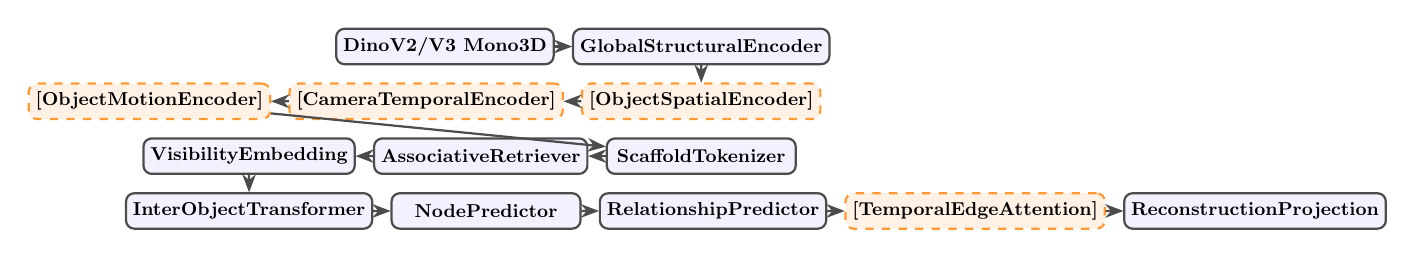
\begin{tikzpicture}[
  scale=0.75, transform shape, >=Stealth,
  block/.style={draw=black!70, rounded corners=3pt, line width=0.8pt, fill=blue!5, minimum width=3.2cm, minimum height=0.6cm, font=\small\bfseries, align=center},
  toggle/.style={draw=orange!80, rounded corners=3pt, line width=0.8pt, fill=orange!10, minimum width=3.2cm, minimum height=0.6cm, font=\small\bfseries, align=center, dashed},
  arrow/.style={->, thick, black!70}
]

\node[block] (mono) {DinoV2/V3 Mono3D};
\node[block, right=0.3cm of mono] (gse) {GlobalStructuralEncoder};
\node[toggle, below=0.3cm of gse] (ose) {[ObjectSpatialEncoder]};
\node[toggle, left=0.3cm of ose] (cte) {[CameraTemporalEncoder]};
\node[toggle, left=0.3cm of cte] (ome) {[ObjectMotionEncoder]};
\node[block, below=0.3cm of ose] (tok) {ScaffoldTokenizer};
\node[block, left=0.3cm of tok] (ret) {AssociativeRetriever};
\node[block, left=0.3cm of ret] (vis) {VisibilityEmbedding};
\node[block, below=0.3cm of vis] (iot) {InterObjectTransformer};
\node[block, right=0.3cm of iot] (np) {NodePredictor};
\node[block, right=0.3cm of np] (rp) {RelationshipPredictor};
\node[toggle, right=0.3cm of rp] (tea) {[TemporalEdgeAttention]};
\node[block, right=0.3cm of tea] (recon) {ReconstructionProjection};

\draw[arrow] (mono) -- (gse);
\draw[arrow] (gse) -- (ose);
\draw[arrow] (ose) -- (cte);
\draw[arrow] (cte) -- (ome);
\draw[arrow] (ome) -- (tok);
\draw[arrow] (tok) -- (ret);
\draw[arrow] (ret) -- (vis);
\draw[arrow] (vis) -- (iot);
\draw[arrow] (iot) -- (np);
\draw[arrow] (np) -- (rp);
\draw[arrow] (rp) -- (tea);
\draw[arrow] (tea) -- (recon);

\end{tikzpicture}
\caption{The WorldWise pipeline.  Bracketed modules (orange, dashed) are togglable via configuration flags for systematic ablation studies.  The core MWAE pathway (solid blue) is always active.}
\label{fig:pipeline_worldwise}
\end{figure}

% ====================================================================================
\section{Structural and Contextual Encoders}
\label{sec:encoders}
% ====================================================================================

WorldWise reuses the same shared encoder modules as the baseline methods (W-STTran, W-DsgDetr families), described in detail below.  Three of the four encoders are togglable, enabling systematic ablation while keeping the MWAE core intact.

\subsection{GlobalStructuralEncoder}

The \emph{GlobalStructuralEncoder} converts world-frame 3D oriented bounding boxes into per-object structural tokens, grounding every object in the persistent geometric scaffold.  An OBB is parameterized by its $8$ corner vertices $\mat{C}_n \in \mR^{8 \times 3}$.  We first center each box to obtain a translation-invariant local geometry:
\begin{align}
    \bar{\mat{c}}_n &= \frac{1}{8}\sum_{i=1}^{8}\mat{c}_{n,i} \in \mR^{3}, \label{eq:center} \\
    \tilde{\mat{c}}_{n,i} &= \mat{c}_{n,i} - \bar{\mat{c}}_n \in \mR^{3}, \quad i=1,\dots,8. \label{eq:local}
\end{align}
The local corners are flattened to a 24-dimensional vector and concatenated with the absolute center, yielding a 27-dimensional per-object input.  A shared MLP with ReLU activations and an intermediate LayerNorm produces:
\begin{equation}
    \mat{g}_n = \op{MLP}_{\text{obj}}\bigl([\op{flatten}(\tilde{\mat{c}}_{n,i}) \;\|\; \bar{\mat{c}}_n]\bigr) \in \mR^{d_{\text{struct}}}.
    \label{eq:gse}
\end{equation}
A permutation-invariant global scene summary is also computed via max-pooling over valid objects $\mathcal{V}$:
\begin{equation}
    \mat{g}_{\text{global}} = \op{MLP}_{\text{global}}\!\Bigl(\max_{n \in \mathcal{V}} \mat{g}_n\Bigr) \in \mR^{d_{\text{struct}}}.
    \label{eq:gse_global}
\end{equation}
This module operates in 3D world coordinates rather than 2D image space, enabling WorldWise to reason about full OBB geometry including object orientation and 3D extent---information critical for spatial predicates such as ``in front of'' vs.\ ``beside.''

\subsection{ObjectSpatialEncoder (Togglable)}

WorldSGG involves moving cameras, requiring explicit camera-relative reasoning.  The \emph{ObjectSpatialEncoder} computes view-dependent features from the camera extrinsic matrix $\mat{T} = [\mat{R}\,|\,\boldsymbol{\tau}]$.

\paragraph{Global Camera Token.}  The rotation matrix is converted to its continuous 6D representation (first two columns of $\mat{R}$) and concatenated with the translation:
\begin{equation}
    \mat{c}_{\text{cam}} = \op{MLP}_{\text{cam}}\bigl([\op{6D}(\mat{R}) \;\|\; \boldsymbol{\tau}]\bigr) \in \mR^{d_{\text{camera}}}.
    \label{eq:cam_global}
\end{equation}

\paragraph{Per-Object Camera-Relative Features.}  For each object $n$, we compute camera-relative geometry:
\begin{align}
    \mat{d}_n &= \bar{\mat{c}}_n - \boldsymbol{\tau}, & &\text{(camera-to-object direction)} \label{eq:cam_dir} \\
    \alpha_n &= \hat{\mat{d}}_n \cdot (-\mat{R}_{:,2}), & &\text{(view alignment cosine)} \label{eq:view_align} \\
    \beta_n^{\sin},\,\beta_n^{\cos} &= \hat{\mat{d}}_n \cdot \mat{R}_{:,0},\; \alpha_n. & &\text{(azimuth sin/cos)} \label{eq:azimuth}
\end{align}
These are combined and projected:
\begin{equation}
    \mat{c}_n = \op{MLP}\bigl([\log\|\mat{d}_n\|,\;\alpha_n,\;\beta_n^{\sin},\;\beta_n^{\cos}]\bigr) \in \mR^{d_{\text{camera}}}.
    \label{eq:cam_per_obj}
\end{equation}
This encoding enables the model to understand \emph{why} an object disappeared---left the field of view due to camera motion (recoverable by reversing the trajectory) vs.\ physical occlusion (requiring associative retrieval from memory).

\subsection{CameraTemporalEncoder (Togglable)}

A dedicated ego-motion encoder processes the full sequence of camera poses to capture long-range camera motion patterns (e.g., panning, orbiting).  For consecutive frames $(t{-}1, t)$, the relative pose is computed:
\begin{align}
    \mat{R}_{\text{rel}}^{(t)} &= \mat{R}_t \mat{R}_{t-1}^{\!\top}, \label{eq:rel_rot} \\
    \boldsymbol{\tau}_{\text{rel}}^{(t)} &= \boldsymbol{\tau}_t - \mat{R}_{\text{rel}}^{(t)}\boldsymbol{\tau}_{t-1}. \label{eq:rel_trans}
\end{align}
Each relative pose is encoded via an MLP, augmented with learnable temporal positional embeddings $\mat{e}_{\tau}$, and the full sequence is processed by a self-attention encoder:
\begin{equation}
    \mat{e}_t = \op{EgoAttn}\bigl(\{\op{MLP}([\op{6D}(\mat{R}_{\text{rel}}^{(\tau)}) \;\|\; \boldsymbol{\tau}_{\text{rel}}^{(\tau)}]) + \mat{e}_{\tau}\}_{\tau=0}^{T-1}\bigr),
    \label{eq:ego_motion}
\end{equation}
yielding an ego-motion token $\mat{e}_t \in \mR^{d_{\text{camera}}}$ for each frame.

\subsection{ObjectMotionEncoder (Togglable)}

The \emph{ObjectMotionEncoder} captures 3D object dynamics directly from world-frame OBB centers:
\begin{align}
    \mat{v}_n^{(t)} &= \bar{\mat{c}}_n^{(t)} - \bar{\mat{c}}_n^{(t-1)}, \quad \text{(velocity)} \label{eq:velocity} \\
    \mat{a}_n^{(t)} &= \mat{v}_n^{(t)} - \mat{v}_n^{(t-1)}. \quad \text{(acceleration)} \label{eq:accel}
\end{align}
A camera-relative velocity $\mat{v}_n^{\text{cam}} = \mat{R}^{\!\top}\mat{v}_n$ provides parallax-aware motion signals.  The full 11-dimensional feature vector $[\mat{v}_n,\,\mat{a}_n,\,\|\mat{v}_n\|,\,\mat{v}_n^{\text{cam}},\,\|\mat{v}_n^{\text{cam}}\|]$ is projected via an MLP to produce motion tokens $\mat{\mu}_n^{(t)} \in \mR^{d_{\text{motion}}}$.  The first frame receives a learnable ``no-motion'' embedding.  By operating in 3D world coordinates, these features capture true physical displacement independent of camera motion---essential for distinguishing contact relationships (e.g., ``carrying'' implies co-moving) from spatial coincidence.


% ====================================================================================
\section{ScaffoldTokenizer}
\label{sec:tokenizer}
% ====================================================================================

The \emph{ScaffoldTokenizer} performs \textbf{top-down initialization} of the world graph: every object receives a token at every frame, regardless of visibility.  This contrasts sharply with the bottom-up approach used by the baseline methods, where tokens are initialized only for objects with available visual features (via the LKS memory buffer).

\paragraph{Visual Component.}  For each object $n$ at frame $t$, the visual slot is filled conditionally:
\begin{equation}
    \mat{v}_n^{(t)} = \begin{cases}
        \op{VisProj}(\mat{f}_n^{(t)}) & \text{if visible and not masked}, \\
        \mat{e}_{\text{[MASK]}} & \text{otherwise},
    \end{cases}
    \label{eq:vis_mask}
\end{equation}
where $\op{VisProj}$ is a learned linear projection from $d_{\text{roi}}$ to $d_{\text{visual}}$, and $\mat{e}_{\text{[MASK]}} \in \mR^{d_{\text{visual}}}$ is a learnable mask embedding shared across all objects and frames.

\paragraph{Training-Time Stochastic Masking.}  During training, a fraction $p_{\text{mask}}$ of \emph{visible} objects are artificially masked---their visual features replaced with $\mat{e}_{\text{[MASK]}}$---to force the AssociativeRetriever to learn robust associative recovery.  This ensures the reconstruction loss has non-trivial targets even when few natural occlusions occur.  This augmentation strategy mirrors the random masking in MAE, but targets individual objects rather than image patches, and supplements rather than replaces the natural masking from occlusion.

\paragraph{Token Fusion.}  The token fuses geometry, the visual/mask feature, and any enabled togglable encoders via a linear projection followed by LayerNorm and GELU:
\begin{equation}
    \mat{x}_n^{(t)} = \op{FusionProj}\bigl([\mat{g}_n^{(t)} \;\|\; \mat{v}_n^{(t)} \;\|\; \mat{c}_n^{(t)} \;\|\; \mat{\mu}_n^{(t)} \;\|\; \mat{e}_t]\bigr) \in \mR^{d_{\text{model}}}.
    \label{eq:tokenizer}
\end{equation}
When togglable encoders are disabled, the corresponding slots are zeroed out, preserving the input dimensionality.

% ====================================================================================
\section{AssociativeRetriever}
\label{sec:retriever}
% ====================================================================================

The \emph{AssociativeRetriever} is the core innovation of WorldWise, functioning as the ``decoder'' in the MAE analogy.  It restores masked object states via \textbf{per-object bidirectional cross-attention} across the full video sequence, allowing each object's temporal trace to be completed by attending to time steps where the object was actually observed.

\paragraph{Architecture.}  Each object $n$'s temporal sequence of length $T$ is processed independently by stacked cross-attention layers with pre-norm (LayerNorm before attention and feed-forward network) and GELU activation.  The attention is \emph{asymmetric}: the Query pool spans all frames (visible + masked), while the Key and Value pools are restricted to frames where the object is visible and unmasked, enforced by a visibility padding mask.

\paragraph{View-Aware Bias.}  Camera pose features are additively injected into the Query and Key projections---but \emph{not} Values---to bias the retrieval mechanism toward frames captured from similar viewpoints:
\begin{align}
    \mat{Q}_n &= \mat{X}_n + \mat{W}_q \mat{C}_n, \label{eq:query} \\
    \mat{K}_n &= \mat{X}_n^{\text{vis}} + \mat{W}_k \mat{C}_n^{\text{vis}}, \label{eq:key} \\
    \mat{V}_n &= \mat{X}_n^{\text{vis}}, \label{eq:value}
\end{align}
where $\mat{C}_n$ denotes the per-object camera-relative features from the ObjectSpatialEncoder.  This design is motivated by the observation that visual features are more transferable between nearby camera positions---an object viewed from $30^{\circ}$ should preferentially retrieve its appearance at $35^{\circ}$ rather than $150^{\circ}$.  Keeping camera bias out of Values ensures that the retrieved content remains purely visual, uncontaminated by viewpoint information.

\paragraph{Iterative Key/Value Refinement.}  After each cross-attention layer, the Key and Value representations at visible positions are updated with the evolved Query values:
\begin{equation}
    \mat{k}_n^{(t)} \leftarrow \begin{cases} \mat{q}_n^{(t)} + \op{KProj}(\mat{c}_n^{(t)}) & \text{if visible}, \\ \mat{k}_n^{(t)} & \text{otherwise}. \end{cases}
    \label{eq:kv_update}
\end{equation}
This allows subsequent layers to attend to progressively richer representations, creating an iterative refinement loop.  Each layer thus refines its retrieval targets based on the context accumulated by previous layers, enabling the model to resolve ambiguities that cannot be addressed in a single attention pass.

\paragraph{Masking Semantics.}  The key padding mask ensures that genuinely unseen tokens and artificially masked tokens are excluded from the Key/Value pool identically.  This prevents information leakage during training (where artificially masked objects still have valid features that could be trivially copied) and ensures the retriever learns to operate robustly under both natural and simulated occlusion.

% ====================================================================================
\section{Visibility Embedding and Spatial Reasoning}
\label{sec:vis_iot}
% ====================================================================================

\subsection{Visibility Embedding}

Following retrieval, a learned \emph{VisibilityEmbedding} provides an explicit signal of whether each token position corresponds to a directly observed or a reconstructed object:
\begin{equation}
    \hat{\mat{x}}_n^{(t)} = \mat{x}_n^{(t)} + \mat{e}_{\text{vis}}[\mathbb{1}[\text{vis}(n,t) \wedge \neg\text{masked}(n,t)]],
    \label{eq:vis_emb}
\end{equation}
where $\mat{e}_{\text{vis}} \in \mR^{2 \times d_{\text{model}}}$ contains two learned embeddings (one for effectively visible, one for effectively masked).  Critically, the mask flag uses \emph{effective} visibility: artificially masked objects are treated as occluded.  This prevents a training shortcut where the downstream modules could bypass the retriever by detecting the visibility indicator rather than relying on the quality of the retrieved representation.

\subsection{InterObjectTransformer}

The completed tokens from all $M(t)$ objects at each frame undergo joint spatial reasoning via the \emph{InterObjectTransformer}.  This module adds continuous, pairwise 3D spatial positional encodings that encode the geometric relationships between every pair of objects in the world frame:
\begin{equation}
    \mat{H}^{(t)} = \op{TransformerEncoder}\bigl(\hat{\mat{X}}^{(t)} + \mat{S}^{(t)},\; \text{mask}=\overline{\mat{v}}^{(t)}\bigr).
    \label{eq:iot}
\end{equation}
The spatial PE matrix $\mat{S}^{(t)}$ encodes inter-object distances $d_{ij}$, unit direction vectors $\hat{\mat{d}}_{ij}$, and log-volume ratios $\rho_{ij} = \log V_i - \log V_j$.  Unlike positional encodings in standard transformers, which are additive to token representations, these spatial PEs are applied as \emph{attention biases}, allowing the model to learn geometry-dependent attention patterns without altering the token content.

By operating over the \emph{full world state} (both visible and reconstructed objects), the InterObjectTransformer enables reasoning about relationships that span observed and unobserved entities---the defining capability that distinguishes WorldSGG from standard VidSGG.

% ====================================================================================
\section{Predictors and Cross-View Reconstruction}
\label{sec:predictors}
% ====================================================================================

\subsection{Node Predictor}

A lightweight 2-layer MLP with ReLU activation maps each refined object representation to class logits:
\begin{equation}
    \hat{\mat{y}}_n^{\text{obj}} = \op{MLP}_{\text{node}}(\mat{h}_n) \in \mR^{C_{\text{obj}}}.
    \label{eq:node_pred}
\end{equation}
This module is active only in SGDet and SGCls evaluation modes.

\subsection{Relationship Predictor}

Relationship prediction proceeds in three phases, shared with the baseline methods:

\paragraph{Phase 1: Token Formation.}  For each human--object pair $(p, o)$, a relationship token is formed by concatenating node features, union ROI features $\mat{u}_{po}$ (or a learnable ``no-union'' embedding for unobserved pairs), and CLIP text embeddings indexed by the predicted class:
\begin{equation}
    \mat{r}_{po} = \op{Proj}\bigl([\mat{h}_p \;\|\; \mat{h}_o \;\|\; \mat{u}_{po} \;\|\; \mat{e}_p^{\text{txt}} \;\|\; \mat{e}_o^{\text{txt}}]\bigr) \in \mR^{d_{\text{rel}}}.
    \label{eq:rel_token}
\end{equation}

\paragraph{Phase 2: Intra-Frame Self-Attention.}  All $K_t$ relationship tokens within each frame self-attend to resolve ambiguities (e.g., mutually exclusive contacts):
\begin{equation}
    \mat{R}^{(t)} = \op{RelTransformer}\bigl(\{\mat{r}_{po}\}_{(p,o) \in \mathcal{P}_t}\bigr) \in \mR^{K_t \times d_{\text{rel}}}.
    \label{eq:rel_attn}
\end{equation}

\paragraph{Phase 3: Temporal Edge Attention (Togglable).}  When enabled, the \emph{TemporalEdgeAttention} module regroups relationship tokens by edge identity across frames and applies a temporal transformer encoder:
\begin{equation}
    \tilde{\mat{R}} = \op{TemporalEncoder}\bigl(\mat{R} + \mat{e}_{\tau}\bigr),
    \label{eq:tea}
\end{equation}
providing temporal smoothing and enabling the model to reason about how relationships evolve over time.

\paragraph{Prediction Heads.}  Three independent MLP heads output the final relationship probabilities:
\begin{align}
    \hat{\mat{y}}_{\text{att}} &= \op{MLP}_{\text{att}}(\tilde{\mat{r}}) \in \mR^{3}, & &\text{(attention, mutually exclusive)} \label{eq:att_head} \\
    \hat{\mat{y}}_{\text{spa}} &= \sigma\!\bigl(\op{MLP}_{\text{spa}}(\tilde{\mat{r}})\bigr) \in [0,1]^{6}, & &\text{(spatial, multi-label)} \label{eq:spa_head} \\
    \hat{\mat{y}}_{\text{con}} &= \sigma\!\bigl(\op{MLP}_{\text{con}}(\tilde{\mat{r}})\bigr) \in [0,1]^{17}. & &\text{(contacting, multi-label)} \label{eq:con_head}
\end{align}

\subsection{Cross-View Reconstruction}

A linear projection head maps the fully refined tokens back to the original visual feature space, providing a self-supervised signal that encourages the retriever to faithfully reconstruct object appearance---not just category---through the completion process:
\begin{equation}
    \hat{\mat{f}}_n^{(t)} = \mat{W}_{\text{recon}} \mat{h}_n^{(t)} + \mat{b}_{\text{recon}} \in \mR^{d_{\text{roi}}}.
    \label{eq:recon}
\end{equation}
This reconstruction is evaluated only on \emph{artificially masked} objects (not padding or genuinely unseen objects, which lack meaningful visual targets).  The objective forces the retriever to preserve fine-grained visual cues relevant to relationship prediction (e.g., hand pose for ``holding'' vs.\ ``touching''), ensuring that these nuances survive the completion process.

% ====================================================================================
\section{Loss Function}
\label{sec:loss}
% ====================================================================================

The WorldWise training objective combines four complementary loss terms:
\begin{equation}
    \mathcal{L}_{\text{WorldWise}} = \mathcal{L}_{\text{SG}} + \lambda_{\text{recon}} \cdot \lambda_{\text{dom}} \cdot \mathcal{L}_{\text{recon}} + \mathcal{L}_{\text{sim}} + \lambda_{\text{stab}} \cdot \mathcal{L}_{\text{stab}}.
    \label{eq:total_loss}
\end{equation}

\paragraph{1.\ Scene Graph Loss ($\mathcal{L}_{\text{SG}}$).}  The primary supervision signal combines cross-entropy for the mutually exclusive attention predicate and binary cross-entropy for the multi-label spatial and contacting predicates.  Pairs are split into two supervision buckets:
\begin{equation}
    \mathcal{L}_{\text{SG}} = \mathcal{L}_{r}^{\text{vis}} + \lambda_{\text{vlm}} \cdot \mathcal{L}_{r}^{\text{unseen}},
    \label{eq:sg_loss}
\end{equation}
where $\mathcal{L}_{r}^{\text{vis}}$ uses clean manual annotations for visible-visible pairs, and $\mathcal{L}_{r}^{\text{unseen}}$ uses VLM-generated pseudo-labels for pairs involving at least one unobserved object, weighted by $\lambda_{\text{vlm}}$.

\paragraph{2.\ Reconstruction Loss ($\mathcal{L}_{\text{recon}}$).}  Mean squared error between the predicted and ground-truth DINO features, computed \emph{exclusively} over artificially masked object-frame pairs:
\begin{equation}
    \mathcal{L}_{\text{recon}} = \frac{1}{|\mathcal{M}_{\text{art}}|}\sum_{(t,n) \in \mathcal{M}_{\text{art}}} \|\hat{\mat{f}}_n^{(t)} - \mat{f}_n^{(t)}\|^2,
    \label{eq:recon_loss}
\end{equation}
where $\mathcal{M}_{\text{art}}$ denotes the set of artificially masked (not genuinely unseen) object-frame pairs.  The dominance factor $\lambda_{\text{dom}}$ prevents the reconstruction gradient from being overwhelmed by the scene graph loss in early training.

\paragraph{3.\ Simulated-Unseen Loss ($\mathcal{L}_{\text{sim}}$).}  For artificially masked objects, the model re-predicts relationships using the completed representations and compares against \emph{clean} manual ground truth (since these objects were actually visible):
\begin{equation}
    \mathcal{L}_{\text{sim}} = \frac{1}{|\mathcal{S}|}\sum_{(p,o) \in \mathcal{S}} \bigl[\op{CE}(\hat{\mat{y}}_{\text{att}}, y_{\text{att}}) + \op{BCE}(\hat{\mat{y}}_{\text{spa}}, y_{\text{spa}}) + \op{BCE}(\hat{\mat{y}}_{\text{con}}, y_{\text{con}})\bigr].
    \label{eq:sim_loss}
\end{equation}
This creates a powerful self-supervised signal: the model is trained to predict relationships for objects it \emph{can} see but has been told to pretend are unseen.  Since the ground truth is clean (not VLM pseudo-labels), this provides high-quality gradients for learning the completion-to-prediction pathway.

\paragraph{4.\ Attractor Stability Loss ($\mathcal{L}_{\text{stab}}$, Optional).}  An optional regularizer that encourages enriched object representations to remain close to a slowly-evolving target:
\begin{equation}
    \mathcal{L}_{\text{stab}} = \op{MSE}(\mat{h}_{\text{final}},\, \op{sg}(\mat{h}_{\text{prev}})),
    \label{eq:stability_loss}
\end{equation}
where $\op{sg}(\cdot)$ denotes stop-gradient.  This loss is only active when $\lambda_{\text{stab}} > 0$ and a previous representation $\mat{h}_{\text{prev}}$ is available.

% ====================================================================================
\section{Ablation Configuration}
\label{sec:ablation}
% ====================================================================================

A key advantage of the WorldWise architecture is its support for \textbf{systematic ablation} via configuration flags.  Four modules can be independently toggled without altering the core MWAE pathway (ScaffoldTokenizer $\to$ AssociativeRetriever $\to$ VisibilityEmbedding $\to$ InterObjectTransformer), enabling precise measurement of each module's contribution.

\begin{table}[h]
\centering
\caption{WorldWise configuration flags and their effects.  Each flag can be independently set to \texttt{True} or \texttt{False}.}
\label{tab:ablation_flags}
\begin{tabular}{@{}lp{6.5cm}@{}}
\toprule
\textbf{Configuration Flag} & \textbf{Effect when Disabled} \\
\midrule
\texttt{use\_object\_spatial\_encoder} & Camera-relative position features ($\mat{c}_n$) are zeroed; the tokenizer receives no view-dependent spatial input. \\
\texttt{use\_camera\_temporal} & Ego-motion token ($\mat{e}_t$) is zeroed; the AssociativeRetriever loses view-aware bias for cross-attention. \\
\texttt{use\_object\_motion\_encoder} & Object motion features ($\mat{\mu}_n^{(t)}$) are zeroed; the model relies solely on static geometry and visual features. \\
\texttt{use\_temporal\_edge\_attn} & Relationship tokens are predicted directly from intra-frame self-attention without temporal smoothing. \\
\bottomrule
\end{tabular}
\end{table}

This systematic toggling, combined with three backbone choices (DinoV2-B, DinoV2-L, DinoV3-L) and two evaluation modes (PredCls, SGDet), produces a comprehensive ablation matrix that isolates the contribution of each architectural component.

% ====================================================================================
\section{Algorithm: Forward Pass}
\label{sec:algorithm}
% ====================================================================================

\begin{algorithm}[h]
\caption{WorldWise Forward Pass}
\begin{algorithmic}[1]
\Require $\mat{f}_{\text{all}}$ (visual), $\mat{C}_{\text{all}}$ (OBBs), $\mat{T}_{\text{all}}$ (camera)
\Ensure $\hat{\mat{y}}_{\text{att}}, \hat{\mat{y}}_{\text{spa}}, \hat{\mat{y}}_{\text{con}}$, $\hat{\mat{f}}_{\text{recon}}$
\State $\mat{G}_{\text{all}} \gets \text{GlobalStructuralEncoder}(\mat{C}_{\text{all}})$
\State $\mat{c}_{\text{all}} \gets \text{ObjectSpatialEncoder}(\mat{T}_{\text{all}}, \mat{C}_{\text{all}})$ \Comment{If enabled}
\State $\mat{e}_{\text{all}} \gets \text{CameraTemporalEncoder}(\mat{T}_{\text{all}})$ \Comment{If enabled}
\State $\mat{\mu}_{\text{all}} \gets \text{ObjectMotionEncoder}(\mat{C}_{\text{all}}, \mat{T}_{\text{all}})$ \Comment{If enabled}
\State $\mat{X} \gets \text{ScaffoldTokenizer}(\mat{G}_{\text{all}}, \mat{f}_{\text{all}}, \mat{c}_{\text{all}}, \mat{\mu}_{\text{all}}, \mat{e}_{\text{all}})$
\State $\mat{X}_{\text{ret}} \gets \text{AssociativeRetriever}(\mat{X}, \mat{c}_{\text{all}})$ \Comment{Masked queries $\to$ Visible keys}
\State $\hat{\mat{X}} \gets \mat{X}_{\text{ret}} + \text{VisibilityEmbedding}(\text{mask})$
\State $\mat{H} \gets \text{InterObjectTransformer}(\hat{\mat{X}})$
\State $\hat{\mat{f}}_{\text{recon}} \gets \mat{W}_{\text{recon}} \mat{H} + \mat{b}_{\text{recon}}$ \Comment{Cross-View Reconstruction}
\State $\hat{\mat{Y}}^{\text{obj}} \gets \text{NodePredictor}(\mat{H})$
\State $\mat{R} \gets \text{RelationshipFormationAndSelfAttention}(\mat{H}, \hat{\mat{Y}}^{\text{obj}})$
\State $\tilde{\mat{R}} \gets \text{TemporalEdgeAttention}(\mat{R})$ \Comment{If enabled}
\State $(\hat{\mat{y}}_{\text{att}}, \hat{\mat{y}}_{\text{spa}}, \hat{\mat{y}}_{\text{con}}) \gets \text{PredictionHeads}(\tilde{\mat{R}})$
\State \Return $\hat{\mat{y}}_{\text{att}}, \hat{\mat{y}}_{\text{spa}}, \hat{\mat{y}}_{\text{con}}$, $\hat{\mat{f}}_{\text{recon}}$
\end{algorithmic}
\end{algorithm}

\end{document}

